% Author: Seongjin Lee 
% Hanyang University, Seoul, Korea 
% esos.hanyang.ac.kr 
% 2016-09-20
% note: some slides are adopted from  \url{www.cs.stevens.edu/~jschauma/631A/}
% https://github.com/resourceful/lecture_sysprog/

\documentclass[newPxFont,sthlmFooter,nooffset]{beamer}
\usepackage{kotex}
%\usetheme{sthlm}
\usepackage{../beamer_template/beamerthemesthlm}
\hypersetup{pdfauthor={Seongjin Lee (insight@hanyang.ac.kr)},
            pdfsubject={Lecture Note: System Programming},
            pdfkeywords={Lecture Note, System Programming, class, undergraduate},
            pdfmoddate={D: \pdfdate},
            pdfcreator={Seongjin Lee}}

%\setbeamertemplate{footline}[text line]{%
%    \parbox{\linewidth}{\vspace*{-8pt} \insertsectionhead  \hfill\insertshortauthor\hfill\insertpagenumber}}
%\setbeamertemplate{navigation symbols}{}




\title{System Programming}
\subtitle{Week 7: Signals}
\author[SJL]{Seongjin Lee}
\institute{\href{mailto:insight@hanyang.ac.kr}{insight@hanyang.ac.kr}\\\url{http://esos.hanyang.ac.kr}\\Esos Lab. Hanyang University}
\date{2016-10-19} 

\begin{document}



\frame[plain]{\titlepage} 

\frame[t]{\frametitle{Table of contents}\tableofcontents} 


%---------------------------------------------------------



\begin{frame}[t]
  \frametitle{introduction}
This chapter covers following items
  \begin{itemize}
  \item The concept
  \item Use cases of signal
  \item The problems of earlier implementations
  \item The correct ways
  \end{itemize}

\end{frame}

\section{Signal Concepts}


\begin{frame}[t]
  \frametitle{Signal Concepts}

Every signal has a name that begins with \texttt{SIG} and it is assigned with a positive number defined in \texttt{<signal.h>}
\begin{itemize}
\item \texttt{SIGABRT}: generated when a process calls \texttt{abort} function
\item \texttt{SIGALRM}: generated when a timer set byt \texttt{alarm} function goes off
\item Different versions of \textsc{Unix} have different number of signals
\end{itemize}
\end{frame}

\begin{frame}[t]
  \frametitle{Signal Concepts}
Signal generating conditions
\begin{enumerate}
\item <1-> terminal generated signals (\texttt{DELETE} or \texttt{\^-C} on many systems) causes the interrupt signal (\texttt{SIGINT})
\item <2-> Hardware exceptions generate singals
  \begin{itemize}
  \item <2-> invalid memory reference (\texttt{SIGSEGV})
  \item <2-> I/O completed (\texttt{SIGIO})
  \item <2-> user disconnected from the system (\texttt{SIGHUP})
  \item <2-> detected by HW and the kernel is notified
  \item <2-> kernel generates the appropriate signal for the process
  \end{itemize}
\item <3-> \texttt{kill(2)} function allows a process to send any signal to another process or group (have to be owner, or the superuser)
\item <4-> \texttt{kill(1)} command sends signal to other process
\item <5-> Software conditions can generate signals
\end{enumerate}

\end{frame}

\begin{frame}
  \frametitle{Signal Concepts cont'd}
Signals are asynchronous events that occurs randomly

The process has to tell the kernel ``if and when this signal occurs, do the following''

\uncover<2->{We can tell the kernel to do one of three things}
\begin{enumerate}
\item <2-> \textbf{Ignore the signal} following two can never be ignored: \texttt{SIGKILL} and \texttt{SIGSTOP} 
\item <3-> \textbf{Catch the signal} We tell the kernel to call a customized function whenever the signal occurs
  \begin{itemize}
  \item <3-> if \texttt{SIGCHLD} signal is caught, it means child has terminated
  \item <3-> signal catching function calls \texttt{waitpid} to fetch the child's process ID and termination status
  \end{itemize}
\item <4-> \textbf{Use default action} every signal has a default action
  \begin{itemize}
  \item <4-> the default action for most signals is to terminate the process> 
  \end{itemize}
\end{enumerate}

\end{frame}

\begin{frame}[t]
  \frametitle{Signal Concepts cont'd}
  \begin{figure}[h]
    \centering
    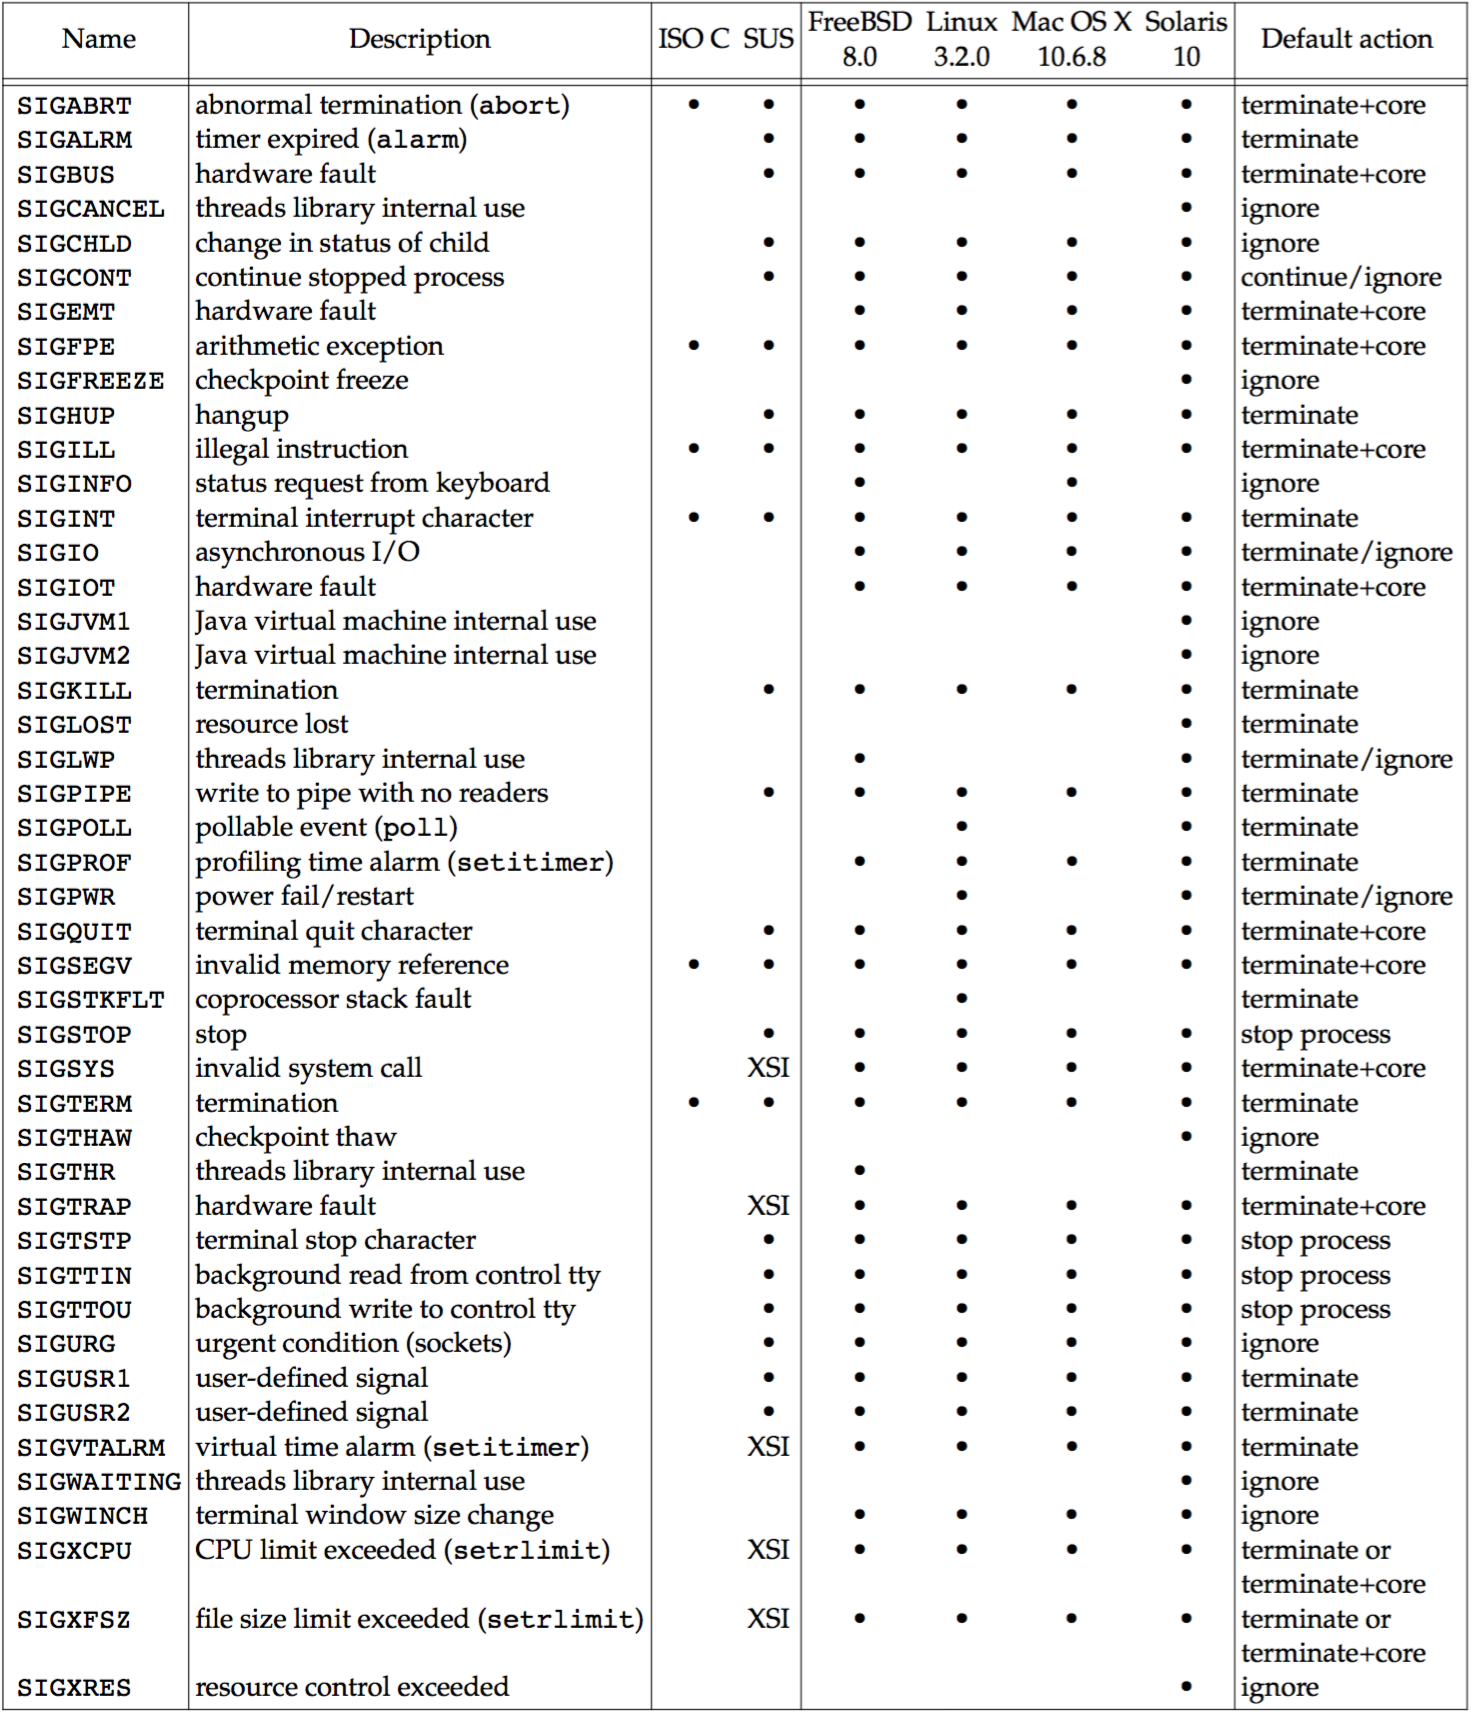
\includegraphics[width=\linewidth,trim={0 15cm 0 0},clip]{figure/fig10-1_unix_sig.png}
    \caption{\textsc{Unix} System signals}
  \end{figure}
\end{frame}

\begin{frame}[fragile,t]
  \frametitle{\texttt{signal} Function}
\begin{codedef}
#include <signal.h> 
void (*signal(int signo, void (*func)(int)))(int); 
// Returns: previous disposition of signal (see following) if OK, SIG_ERR on error
\end{codedef}

\begin{itemize}[ ]
\item \texttt{signo} is name of the signal from the Table 10.1
\item \texttt{func} is
  \begin{itemize}
  \item \texttt{SIG\_IGN} : to ignore the signal
  \item \texttt{SIG\_DFL} : to use the default value
  \item address of a function to be called when the signal occurs---they are called \textit{signal handler} or \textit{signal-catching function}
  \end{itemize}
\end{itemize}
\end{frame}


\begin{frame}[fragile,fragile,allowframebreaks,t]
  \frametitle{Signal Exmple Code: \texttt{codes/usr\_sig.c}}
\lstinputlisting[lineskip=0pt]{codes/usr_sig.c}
\end{frame}



\begin{frame}[fragile,t]
  \frametitle{Signal Exmaples}
invoke the program in the background and use \texttt{kill(1)} to send signal
\begin{codedefnb}
James@maker:codes$ ./usr\_sig &
[2] 4987
James@maker:codes$ kill -USR1 4987
received SIGUSR1
James@maker:codes$ kill -USR2 4987
received SIGUSR2
James@maker:codes$ kill -HUP 4987
received SIGHUP
James@maker:codes$ kill -INT 4987
[2]+  Interrupt: 2            ./usr\_sig 
James@maker:codes$
\end{codedefnb}
\end{frame}




\begin{frame}[t]
  \frametitle{\texttt{signal} Function}
At process creation
\begin{itemize}
\item When a process calls \texttt{fork}, the child inherits the parents signal disposition
\item Child starts off with copy of the parent's memory image
\item the address of a signal-catching function has meaning in the child
\end{itemize}
\end{frame}



\section{The issues}

\begin{frame}[t]
  \frametitle{Unreliable Signals}
In earlier versions of \textsc{Unix} system, signals were unreliable

\begin{enumerate}
\item <2-> signals get lost: signal occurs and the process never know about it
\item  <3-> window of time---after the signal has occured, but before the call to \texttt{signal} in the signal handler---when the interrupt signal could occur another time. The second signal would cause the default action to occur (terminate the process)
\item <4-> little control over a signal: unable to turn a signal off when it didn't want the signal to occur. All it can do is to catch or ignore the signal.
\end{enumerate}
\end{frame}

\begin{frame}[t]
  \frametitle{Interrupted System Calls cont'd}
The slow system calls are those that can block forever
\begin{itemize}
\item reads (for pipes, terminal devices, and network devices) that can block the caller
\item writes that can block the caller forever if the data can't be accepted immediately
\item open on a certain file types (terminal device) that block the caller until some condition occurs
\item the \texttt{pause} and \texttt{wait} function
\item certain \texttt{ioctl} operations
\item some of interprocess communication function
\end{itemize}

\end{frame}

\begin{frame}[fragile,t]
  \frametitle{Interrupted System Calls cont'd}
The problem with interrupted system calls is that error returns must be explicit

\begin{codedef}
again:
    if ((n = read(fd, buf, BUFFSIZE)) < 0 ) {
        if (errno == EINTR)
            goto again; /* just an interrupted system call */
        /* handle other errors */
    }
\end{codedef}

The solution of 4.2BSD was to introduce the automatic restaring of \texttt{ioctl}, \texttt{read}, \texttt{readv}, \texttt{write}, \texttt{writev}, \texttt{wait}, and \texttt{waitpid}

\end{frame}



\begin{frame}[fragile,t]
  \frametitle{Reentrant Functions}
\begin{block}{Reentrant Functions}
Reentrant fuctions are guarnateed to be safe to call from within a signal hanlder.   They are also called \textit{async-signal safe}. As a general rule, when calling the reentrant  functions from a signal handler, we should save and restore \texttt{errno}.
\end{block}

\uncover<2-> {Scenario}
\begin{enumerate}
\item <2-> while process is running, it catches a signal. process is temporarily interrupted by the signal handler
\item <3-> instructions in signal handler executes, the returns
\item <4-> upon return of signal handler, the process continues to run
\end{enumerate}

\uncover<5-> {The problem is that signal handler can't tell whether a process was in the middle of execution. \textit{The result becomes unpredictable}}
\end{frame}

\begin{frame}
  \frametitle{Reentrant Functions cont'd}  
  \begin{figure}[h]
    \centering
    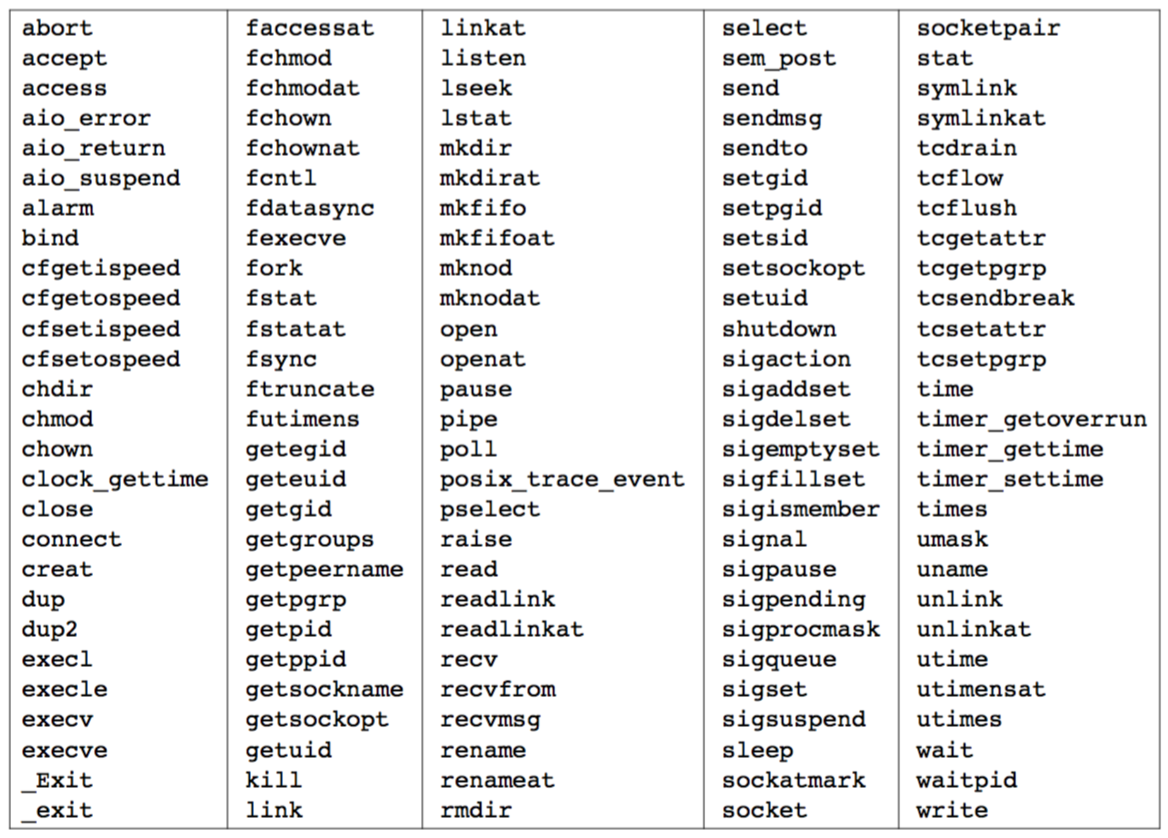
\includegraphics[height=0.87\textheight]{figure/fig10-4_reentrant.png}
    \caption{Reentrant functions that may be called from a signal handler}
  \end{figure}
\end{frame}


\begin{comment}
  \begin{frame}[fragile,t]
    \frametitle{SIGCLD Semantics}
    Beware the semantics of \texttt{SIGCLD} and \texttt{SIGCHLD} is
    different

    refer to section 10.7 of the text
  \end{frame}

\end{comment}


\begin{frame}[fragile,t]
  \frametitle{Reliable-Singnal Teminology and Semantics}

\begin{itemize}
\item  \textbf{a signal is \textit{generated} (or sent) for a process } when the event that causes the signal occurs
  \begin{itemize}
  \item  \footnotesize The event can be hardware exception, software condition, a terminal-generated signal, or a call to the \texttt{kill} function
  \item  \footnotesize when the signal is generated, the kernel usually sets a flag of some form in the process table
  \end{itemize}
\item <2-> \textbf{a signal is \textit{delivered} to a process} when the action for a signal is taken
  \begin{itemize}
  \item <2-> \footnotesize during the time between the generation of a signal and its delivery, the signal is said to be \textbf{\textit{pending}}
  \end{itemize}
\item <3-> \textbf{a process has the option of \textit{blocking} the delievery of a signal}
\item <4-> signals are \textbf{\textit{queued}} when system delievers signals
\item <5-> POSIX.1 does not specify the order if more than one signal is ready to be delievered to a process
\item <6-> \textbf{each process has a \textit{signal mask}} that defines the set of singals currently blocked for delievery to that process
\item <7-> POSIX.1 defines a data type \texttt{sigset\_t} that holds a \textbf{\textit{signal set}}

\end{itemize}

  
\end{frame}




\section{Use cases of signal}



\begin{frame}[fragile,t]
  \frametitle{\texttt{kill} and \texttt{raise} Functions}
\texttt{kill} function sends a signal to a process or a group of processes

\texttt{raise} function allows a process to send a signal to itself

\begin{codedef}
#include <signal.h>
int kill(pid_t pid, int signo); 
int raise(int signo);
// Both return: 0 if OK, −1 on error
\end{codedef}

{\hfill \texttt{raise(signo);} == \texttt{kill(getpid(), singo);}\hfill}

\begin{itemize}
\item \texttt{pid>0} sends signal to \texttt{pid}
\item \texttt{pid==0} sends signal to all prosesses in process group ID of the sender
\item \texttt{pid<0} The signal is sent to all process in process group ID of $|pid|$
\item \texttt{pid==-1} send signal to all processes on the system for which the sender has permission to send the signal
\end{itemize}
\end{frame}



\begin{frame}[fragile,t]
  \frametitle{\texttt{alarm} Function}
\texttt{alarm} function allows us to set a time that will expire at a specified time in the future. When the timer expires, the \texttt{SIGALRM} signal is generated
\begin{codedef}
#include <unistd.h>
unsigned int alarm(unsigned int seconds);
// Returns: 0 or number of seconds until previously set alarm  
\end{codedef}

\begin{itemize}
\item only one of alarm clocks per process
\item if previously registered alarm clock has not expired, the number of seconds left for that alarm clock is returned as the value of this function
\item if previous alarm is not expired and \textit{seconds} value is \texttt{0}, the previous alarm is cacled
\item most processes using alarm, catches this signal
\end{itemize}
\end{frame}

\begin{frame}[fragile,t]
  \frametitle{\texttt{pause} Function}

\texttt{pause} function suspends the calling process until a signal is caught
\begin{codedef}
#include <unistd.h>
int pause(void);
// Returns: −1 with errno set to EINTR
\end{codedef}

\end{frame}

\begin{frame}[fragile,t]
  \frametitle{\texttt{alarm} and \texttt{pause} Functions Example}
\texttt{codes/sleep-pause.c}
\lstinputlisting[lineskip=0pt]{codes/sleep-pause.c}
\end{frame}

\begin{frame}[fragile,t]
  \frametitle{\texttt{alarm} and \texttt{pause} Functions Example}
There are three problems in the code
\begin{enumerate}
\item <2-> if the caller already has an alarm set, that alarm is erased by the first call to \texttt{alarm}
  \begin{itemize}
  \item  we have to check the return value of \texttt{alarm}, and make sure we wait only until the existing alarm expires
  \end{itemize}
\item <3-> disposition for \texttt{SIGALRM} is modified
  \begin{itemize}
  \item if others are going to use this call, make sure the function is restored after use
  \end{itemize}
\item <4-> there is race condition between the first call to \texttt{alarm} and the call to \texttt{puase}
  \begin{itemize}
  \item  use \texttt{setjmp} or \texttt{sigprocmask} with \texttt{sigsuspend}
  \end{itemize}
\end{enumerate}
\end{frame}


\begin{frame}[fragile,t]
  \frametitle{ Example cont'd  \texttt{codes/sleep-pause2.c}}


to avoid race condition SVR2 used \texttt{setjmp} and \texttt{longjmp}
\lstinputlisting[lineskip=-3pt]{codes/sleep-pause2.c}

\end{frame}


\begin{frame}[fragile,t,allowframebreaks]
  \frametitle{Example cont'd \texttt{codes/tsleep.c}}
There is subtle problem with \texttt{sleep2} function when it interacts with other signals

In this example, we are trying to make it execute longer than 5 seconds (the argument to \texttt{sleep2()}

\lstinputlisting[lineskip=-3pt]{codes/tsleep.c}
\end{frame}


\begin{frame}[fragile,t]
  \frametitle{Example cont'd \texttt{codes/tsleep.c}}
\texttt{make tsleep}

We execute the program by \texttt{./tsleep} and interrupt the sleep by typing in the interrupt character

\begin{columns}[t]
\begin{column}{0.5\linewidth}
\begin{codedefnb}
James@maker:codes$ time ./tsleep
sleep2 returned: 0

real	0m5.014s
user	0m0.005s
sys	0m0.007s
\end{codedefnb}
\end{column}
\begin{column}{0.5\linewidth}
\begin{codedefnb}
James@maker:codes$ time ./tsleep
^C
sig_int starting
sleep2 returned: 0

real	0m5.008s
user	0m4.590s
sys	0m0.023s
\end{codedefnb}
\end{column}
\end{columns}

we can see that the \texttt{longjmp} from the \texttt{sleep2} aborted the other signal handler, \texttt{sig\_int}, even though it wasn't finished
\end{frame}


\begin{comment}
  \begin{frame}[fragile,t,allowframebreaks]
    \frametitle{Example cont'd}
    analyze Fig 10.10 and Fig 10.11

  \end{frame}
\end{comment}




\begin{frame}[fragile,t]
  \frametitle{Signal Sets}
We need a data type ot represent multiple signals---\textit{signal set}

\begin{codedef}
#include <signal.h>
int sigemptyset(sigset_t *set);
int sigfillset(sigset_t *set);
int sigaddset(sigset_t *set, int signo); 
int sigdelset(sigset_t *set, int signo);
// All four return: 0 if OK, −1 on error 
int sigismember(const sigset_t *set, int signo);
// Returns: 1 if true, 0 if false, −1 on error
\end{codedef}

\begin{itemize}
\item \footnotesize \texttt{sigemptyset()} initializes the signal set pointed to by set so that all signals are \textit{excluded}
\item \footnotesize \texttt{sigfillset()} initializes the signal set
\item \footnotesize all applications have to call either \texttt{sigemptyset} or \texttt{sigfillset} once for each signal set, before using signal set
\item \footnotesize \texttt{sigaddset} adds a single signal to an existing set
\item \footnotesize \texttt{sigdelset} removes a single signal from a set
\end{itemize}

\end{frame}








\begin{frame}[fragile,t,allowframebreaks]
  \frametitle{Signal Sets cont'd}
An implementation of \texttt{sigaddset}, \texttt{sigdelset}, and \texttt{sigismember}
\lstinputlisting[lineskip=0pt]{codes/setops.c}

POSIX.1 requires us to check the signal number argument for validity and to set \texttt{errno} if it si invalid
\end{frame}



\begin{frame}[fragile,t]
  \frametitle{\texttt{sigprocmask} Function}
A process can \textit{examine} its signal mask, \textit{change} its signal mask, \textit{or perform both} operations by calling following function

\begin{codedef}
#include <signal.h>
int sigprocmask(int how, const sigset_t *restrict set, 
                sigset_t *restrict oset);
// Returns: 0 if OK, −1 on erro    
\end{codedef}
\end{frame}



\begin{frame}[fragile,t]
  \frametitle{\texttt{sigprocmask} Function}
\begin{codedef}
#include <signal.h>
int sigprocmask(int how, const sigset_t *restrict set, 
                sigset_t *restrict oset);
// Returns: 0 if OK, −1 on erro    
\end{codedef}
\end{frame}



\begin{frame}[fragile,t]
  \frametitle{\texttt{sigpending} Function}
  
\end{frame}



\begin{frame}[fragile,t]
  \frametitle{\texttt{sigaction} Function}
  
\end{frame}


\begin{frame}[fragile,t]
  \frametitle{\texttt{segsetjmp} and \texttt{siglongjmp} Functions}
  
\end{frame}


\begin{frame}[fragile,t]
  \frametitle{\texttt{sigsuspend} Function}
  
\end{frame}



\begin{frame}[fragile,t]
  \frametitle{\texttt{abort} Function}
  
\end{frame}


\begin{frame}[fragile,t]
  \frametitle{\texttt{system} Function}
  
\end{frame}


\begin{frame}[fragile,t]
  \frametitle{\texttt{sleep}, \texttt{nanosleep},  and \texttt{clock\_nanosleep} Functions}
  
\end{frame}


\begin{frame}[fragile,t]
  \frametitle{\texttt{sigqueue} Function}
  
\end{frame}


\begin{frame}[fragile,t]
  \frametitle{Job-Control Signals}
  
\end{frame}



\begin{frame}[fragile,t]
  \frametitle{Signal Names and Numbers}
  
\end{frame}

%---------------------------------------------------------
\section{Last Words}

\begin{frame}[t]
  \frametitle{Last Words}
\begin{itemize}
\item Prepare for Exam
\end{itemize}
\end{frame}

\end{document}
